% Options for packages loaded elsewhere
% Options for packages loaded elsewhere
\PassOptionsToPackage{unicode}{hyperref}
\PassOptionsToPackage{hyphens}{url}
\PassOptionsToPackage{dvipsnames,svgnames,x11names}{xcolor}
%
\documentclass[
  letterpaper,
  DIV=11,
  numbers=noendperiod]{scrreprt}
\usepackage{xcolor}
\usepackage{amsmath,amssymb}
\setcounter{secnumdepth}{5}
\usepackage{iftex}
\ifPDFTeX
  \usepackage[T1]{fontenc}
  \usepackage[utf8]{inputenc}
  \usepackage{textcomp} % provide euro and other symbols
\else % if luatex or xetex
  \usepackage{unicode-math} % this also loads fontspec
  \defaultfontfeatures{Scale=MatchLowercase}
  \defaultfontfeatures[\rmfamily]{Ligatures=TeX,Scale=1}
\fi
\usepackage{lmodern}
\ifPDFTeX\else
  % xetex/luatex font selection
\fi
% Use upquote if available, for straight quotes in verbatim environments
\IfFileExists{upquote.sty}{\usepackage{upquote}}{}
\IfFileExists{microtype.sty}{% use microtype if available
  \usepackage[]{microtype}
  \UseMicrotypeSet[protrusion]{basicmath} % disable protrusion for tt fonts
}{}
\makeatletter
\@ifundefined{KOMAClassName}{% if non-KOMA class
  \IfFileExists{parskip.sty}{%
    \usepackage{parskip}
  }{% else
    \setlength{\parindent}{0pt}
    \setlength{\parskip}{6pt plus 2pt minus 1pt}}
}{% if KOMA class
  \KOMAoptions{parskip=half}}
\makeatother
% Make \paragraph and \subparagraph free-standing
\makeatletter
\ifx\paragraph\undefined\else
  \let\oldparagraph\paragraph
  \renewcommand{\paragraph}{
    \@ifstar
      \xxxParagraphStar
      \xxxParagraphNoStar
  }
  \newcommand{\xxxParagraphStar}[1]{\oldparagraph*{#1}\mbox{}}
  \newcommand{\xxxParagraphNoStar}[1]{\oldparagraph{#1}\mbox{}}
\fi
\ifx\subparagraph\undefined\else
  \let\oldsubparagraph\subparagraph
  \renewcommand{\subparagraph}{
    \@ifstar
      \xxxSubParagraphStar
      \xxxSubParagraphNoStar
  }
  \newcommand{\xxxSubParagraphStar}[1]{\oldsubparagraph*{#1}\mbox{}}
  \newcommand{\xxxSubParagraphNoStar}[1]{\oldsubparagraph{#1}\mbox{}}
\fi
\makeatother

\usepackage{color}
\usepackage{fancyvrb}
\newcommand{\VerbBar}{|}
\newcommand{\VERB}{\Verb[commandchars=\\\{\}]}
\DefineVerbatimEnvironment{Highlighting}{Verbatim}{commandchars=\\\{\}}
% Add ',fontsize=\small' for more characters per line
\usepackage{framed}
\definecolor{shadecolor}{RGB}{241,243,245}
\newenvironment{Shaded}{\begin{snugshade}}{\end{snugshade}}
\newcommand{\AlertTok}[1]{\textcolor[rgb]{0.68,0.00,0.00}{#1}}
\newcommand{\AnnotationTok}[1]{\textcolor[rgb]{0.37,0.37,0.37}{#1}}
\newcommand{\AttributeTok}[1]{\textcolor[rgb]{0.40,0.45,0.13}{#1}}
\newcommand{\BaseNTok}[1]{\textcolor[rgb]{0.68,0.00,0.00}{#1}}
\newcommand{\BuiltInTok}[1]{\textcolor[rgb]{0.00,0.23,0.31}{#1}}
\newcommand{\CharTok}[1]{\textcolor[rgb]{0.13,0.47,0.30}{#1}}
\newcommand{\CommentTok}[1]{\textcolor[rgb]{0.37,0.37,0.37}{#1}}
\newcommand{\CommentVarTok}[1]{\textcolor[rgb]{0.37,0.37,0.37}{\textit{#1}}}
\newcommand{\ConstantTok}[1]{\textcolor[rgb]{0.56,0.35,0.01}{#1}}
\newcommand{\ControlFlowTok}[1]{\textcolor[rgb]{0.00,0.23,0.31}{\textbf{#1}}}
\newcommand{\DataTypeTok}[1]{\textcolor[rgb]{0.68,0.00,0.00}{#1}}
\newcommand{\DecValTok}[1]{\textcolor[rgb]{0.68,0.00,0.00}{#1}}
\newcommand{\DocumentationTok}[1]{\textcolor[rgb]{0.37,0.37,0.37}{\textit{#1}}}
\newcommand{\ErrorTok}[1]{\textcolor[rgb]{0.68,0.00,0.00}{#1}}
\newcommand{\ExtensionTok}[1]{\textcolor[rgb]{0.00,0.23,0.31}{#1}}
\newcommand{\FloatTok}[1]{\textcolor[rgb]{0.68,0.00,0.00}{#1}}
\newcommand{\FunctionTok}[1]{\textcolor[rgb]{0.28,0.35,0.67}{#1}}
\newcommand{\ImportTok}[1]{\textcolor[rgb]{0.00,0.46,0.62}{#1}}
\newcommand{\InformationTok}[1]{\textcolor[rgb]{0.37,0.37,0.37}{#1}}
\newcommand{\KeywordTok}[1]{\textcolor[rgb]{0.00,0.23,0.31}{\textbf{#1}}}
\newcommand{\NormalTok}[1]{\textcolor[rgb]{0.00,0.23,0.31}{#1}}
\newcommand{\OperatorTok}[1]{\textcolor[rgb]{0.37,0.37,0.37}{#1}}
\newcommand{\OtherTok}[1]{\textcolor[rgb]{0.00,0.23,0.31}{#1}}
\newcommand{\PreprocessorTok}[1]{\textcolor[rgb]{0.68,0.00,0.00}{#1}}
\newcommand{\RegionMarkerTok}[1]{\textcolor[rgb]{0.00,0.23,0.31}{#1}}
\newcommand{\SpecialCharTok}[1]{\textcolor[rgb]{0.37,0.37,0.37}{#1}}
\newcommand{\SpecialStringTok}[1]{\textcolor[rgb]{0.13,0.47,0.30}{#1}}
\newcommand{\StringTok}[1]{\textcolor[rgb]{0.13,0.47,0.30}{#1}}
\newcommand{\VariableTok}[1]{\textcolor[rgb]{0.07,0.07,0.07}{#1}}
\newcommand{\VerbatimStringTok}[1]{\textcolor[rgb]{0.13,0.47,0.30}{#1}}
\newcommand{\WarningTok}[1]{\textcolor[rgb]{0.37,0.37,0.37}{\textit{#1}}}

\usepackage{longtable,booktabs,array}
\usepackage{calc} % for calculating minipage widths
% Correct order of tables after \paragraph or \subparagraph
\usepackage{etoolbox}
\makeatletter
\patchcmd\longtable{\par}{\if@noskipsec\mbox{}\fi\par}{}{}
\makeatother
% Allow footnotes in longtable head/foot
\IfFileExists{footnotehyper.sty}{\usepackage{footnotehyper}}{\usepackage{footnote}}
\makesavenoteenv{longtable}
\usepackage{graphicx}
\makeatletter
\newsavebox\pandoc@box
\newcommand*\pandocbounded[1]{% scales image to fit in text height/width
  \sbox\pandoc@box{#1}%
  \Gscale@div\@tempa{\textheight}{\dimexpr\ht\pandoc@box+\dp\pandoc@box\relax}%
  \Gscale@div\@tempb{\linewidth}{\wd\pandoc@box}%
  \ifdim\@tempb\p@<\@tempa\p@\let\@tempa\@tempb\fi% select the smaller of both
  \ifdim\@tempa\p@<\p@\scalebox{\@tempa}{\usebox\pandoc@box}%
  \else\usebox{\pandoc@box}%
  \fi%
}
% Set default figure placement to htbp
\def\fps@figure{htbp}
\makeatother





\setlength{\emergencystretch}{3em} % prevent overfull lines

\providecommand{\tightlist}{%
  \setlength{\itemsep}{0pt}\setlength{\parskip}{0pt}}



 


\KOMAoption{captions}{tableheading}
\makeatletter
\@ifpackageloaded{bookmark}{}{\usepackage{bookmark}}
\makeatother
\makeatletter
\@ifpackageloaded{caption}{}{\usepackage{caption}}
\AtBeginDocument{%
\ifdefined\contentsname
  \renewcommand*\contentsname{Table of contents}
\else
  \newcommand\contentsname{Table of contents}
\fi
\ifdefined\listfigurename
  \renewcommand*\listfigurename{List of Figures}
\else
  \newcommand\listfigurename{List of Figures}
\fi
\ifdefined\listtablename
  \renewcommand*\listtablename{List of Tables}
\else
  \newcommand\listtablename{List of Tables}
\fi
\ifdefined\figurename
  \renewcommand*\figurename{Figure}
\else
  \newcommand\figurename{Figure}
\fi
\ifdefined\tablename
  \renewcommand*\tablename{Table}
\else
  \newcommand\tablename{Table}
\fi
}
\@ifpackageloaded{float}{}{\usepackage{float}}
\floatstyle{ruled}
\@ifundefined{c@chapter}{\newfloat{codelisting}{h}{lop}}{\newfloat{codelisting}{h}{lop}[chapter]}
\floatname{codelisting}{Listing}
\newcommand*\listoflistings{\listof{codelisting}{List of Listings}}
\makeatother
\makeatletter
\makeatother
\makeatletter
\@ifpackageloaded{caption}{}{\usepackage{caption}}
\@ifpackageloaded{subcaption}{}{\usepackage{subcaption}}
\makeatother
\usepackage{bookmark}
\IfFileExists{xurl.sty}{\usepackage{xurl}}{} % add URL line breaks if available
\urlstyle{same}
\hypersetup{
  pdftitle={PTR5932 - Introdução à Ciência de Dados Geoespaciais},
  pdfauthor={Diego Bogado Tomasiello},
  colorlinks=true,
  linkcolor={blue},
  filecolor={Maroon},
  citecolor={Blue},
  urlcolor={Blue},
  pdfcreator={LaTeX via pandoc}}


\title{PTR5932 - Introdução à Ciência de Dados Geoespaciais}
\author{Diego Bogado Tomasiello}
\date{2026-09-18}
\begin{document}
\maketitle

\renewcommand*\contentsname{Table of contents}
{
\hypersetup{linkcolor=}
\setcounter{tocdepth}{2}
\tableofcontents
}

\bookmarksetup{startatroot}

\chapter*{Apresentação}\label{apresentauxe7uxe3o}
\addcontentsline{toc}{chapter}{Apresentação}

\markboth{Apresentação}{Apresentação}

Autor: Diego Bogado Tomasiello

Data: 18/09/2026

Vivemos em uma era de abundância de dados sem precedentes. O avanço
acelerado das tecnologias de informação e comunicação transformou a
forma como registramos, analisamos e compreendemos os fenômenos ao nosso
redor, gerando um volume maciço de informações que trazem consigo um
elemento fundamental: a localização geográfica. No planejamento, na
operação e na gestão dos sistemas de transportes e da infraestrutura
urbana, essa dimensão espacial pode permitir desvendar padrões complexos
da dinâmica territorial.

No entanto, a mera disponibilidade de dados geoespaciais não garante sua
utilidade. Um dos desafios na academia e no mundo corporativo é a
capacidade de transformar grandes volumes de dados geoespaciais em
conhecimento estruturado. É nesse cenário desafiador que se insere este
livro, concebido como o material didático de apoio para a disciplina
PTR-5932: Introdução à Ciência de Dados Geoespaciais, do Programa de
Pós-Graduação em Engenharia de Transportes da Escola Politécnica da
Universidade de São Paulo (USP).

Este material foi estruturado especificamente para preencher uma lacuna:
a necessidade de uma formação introdutória que forneça fundamentos
teóricos e instrumentais para a organização, manipulação e representação
de dados geoespaciais. Destinado a estudantes de mestrado, doutorado,
pesquisadores e profissionais de áreas correlatas, o material tem como
objetivo construir uma base conceitual que dê segurança e autonomia para
que, em etapas posteriores de suas trajetórias, os leitores possam
avançar para a construção de modelos e análises espaciais.

Para atingir esse objetivo, o material apresenta laboratórios didáticos
com aplicações na linguagem de programação R.

\section*{Organização do material}\label{organizauxe7uxe3o-do-material}
\addcontentsline{toc}{section}{Organização do material}

\markright{Organização do material}

\begin{longtable}[]{@{}
  >{\raggedright\arraybackslash}p{(\linewidth - 2\tabcolsep) * \real{0.5360}}
  >{\raggedright\arraybackslash}p{(\linewidth - 2\tabcolsep) * \real{0.4640}}@{}}
\toprule\noalign{}
\begin{minipage}[b]{\linewidth}\raggedright
Aula
\end{minipage} & \begin{minipage}[b]{\linewidth}\raggedright
Descrição
\end{minipage} \\
\midrule\noalign{}
\endhead
\bottomrule\noalign{}
\endlastfoot
\begin{minipage}[t]{\linewidth}\raggedright
\begin{enumerate}
\def\labelenumi{\arabic{enumi}.}
\tightlist
\item
  Introdução
\end{enumerate}
\end{minipage} & Instalação do R e do RStudio. Apresentação da interface
do RStudio, sintaxe da linguagem e instalação de pacotes. \\
\begin{minipage}[t]{\linewidth}\raggedright
\begin{enumerate}
\def\labelenumi{\arabic{enumi}.}
\setcounter{enumi}{1}
\tightlist
\item
  Sistemas de Referência e Projeções Cartográficas
\end{enumerate}
\end{minipage} & Transformação entre Sistemas de Referência e Projeções
Cartográficas. \\
\begin{minipage}[t]{\linewidth}\raggedright
\begin{enumerate}
\def\labelenumi{\arabic{enumi}.}
\setcounter{enumi}{2}
\tightlist
\item
  Dados espaciais: tipos, estruturas, formas de representação e formatos
  de armazenamento
\end{enumerate}
\end{minipage} & Leitura de diferentes formatos de arquivo no R \\
\begin{minipage}[t]{\linewidth}\raggedright
\begin{enumerate}
\def\labelenumi{\arabic{enumi}.}
\setcounter{enumi}{3}
\tightlist
\item
  Dados de entrada em SIG: Infraestruturas de Dados Espaciais, Censos,
  Pesquisas Origem e Destino, VGI, Geocodificação, GNSS etc.
\end{enumerate}
\end{minipage} & Pacotes para leitura de diferentes formatos de dados,
tratamento topológico e geocodificação de dados. \\
\begin{minipage}[t]{\linewidth}\raggedright
\begin{enumerate}
\def\labelenumi{\arabic{enumi}.}
\setcounter{enumi}{4}
\tightlist
\item
  Operações espaciais: buffer, clip, dissolve, intersect, union etc.
\end{enumerate}
\end{minipage} & Principais operações de sobreposição e proximidade \\
\begin{minipage}[t]{\linewidth}\raggedright
\begin{enumerate}
\def\labelenumi{\arabic{enumi}.}
\setcounter{enumi}{5}
\tightlist
\item
  Manipulação de dados raster: álgebra de mapas
\end{enumerate}
\end{minipage} & Leitura, escrita e operações espaciais (locais, focais,
zonais e globais) com dados raster \\
\begin{minipage}[t]{\linewidth}\raggedright
\begin{enumerate}
\def\labelenumi{\arabic{enumi}.}
\setcounter{enumi}{6}
\tightlist
\item
  Modelagem de redes de transportes: redes em SIG e em R (r5r)
\end{enumerate}
\end{minipage} & Princípios de modelagem de redes de transporte em SIG e
em R usando o pacote r5r \\
\begin{minipage}[t]{\linewidth}\raggedright
\begin{enumerate}
\def\labelenumi{\arabic{enumi}.}
\setcounter{enumi}{7}
\tightlist
\item
  Design e produção de mapas
\end{enumerate}
\end{minipage} & Produção de mapas utilizando o pacote cowplot \\
\end{longtable}

\bookmarksetup{startatroot}

\chapter{Aula 01}\label{aula-01}

Pré-requisitos:

\begin{itemize}
\tightlist
\item
  Instalar o \href{https://cran.r-project.org}{R}
\item
  Instalar o \href{https://posit.co/downloads}{RStudio}
\end{itemize}

Instalar os pacotes: -
\href{https://cran.r-project.org/web/packages/sf/}{\texttt{sf}} -
\href{https://cran.r-project.org/package=terra}{\texttt{terra}} -
\href{https://cran.r-project.org/web/packages/dplyr/}{\texttt{dplyr}} -
\href{https://cran.r-project.org/web/packages/data.table/}{\texttt{data.table}}
-
\href{https://cran.r-project.org/web/packages/mapview/}{\texttt{mapview}}
-
\href{https://cran.r-project.org/web/packages/osmdata/}{\texttt{osmdata}}
- \href{https://cran.r-project.org/web/packages/geobr/}{\texttt{geobr}}
-
\href{https://cran.r-project.org/web/packages/geocodebr/}{\texttt{geocodebr}}

\section{Interface do RStudio}\label{interface-do-rstudio}

Após instalar, em sequencia, o R e o RStudio, abra o RStudio e observe a
sua interface (Figura 01).

\begin{figure}[H]

{\centering \pandocbounded{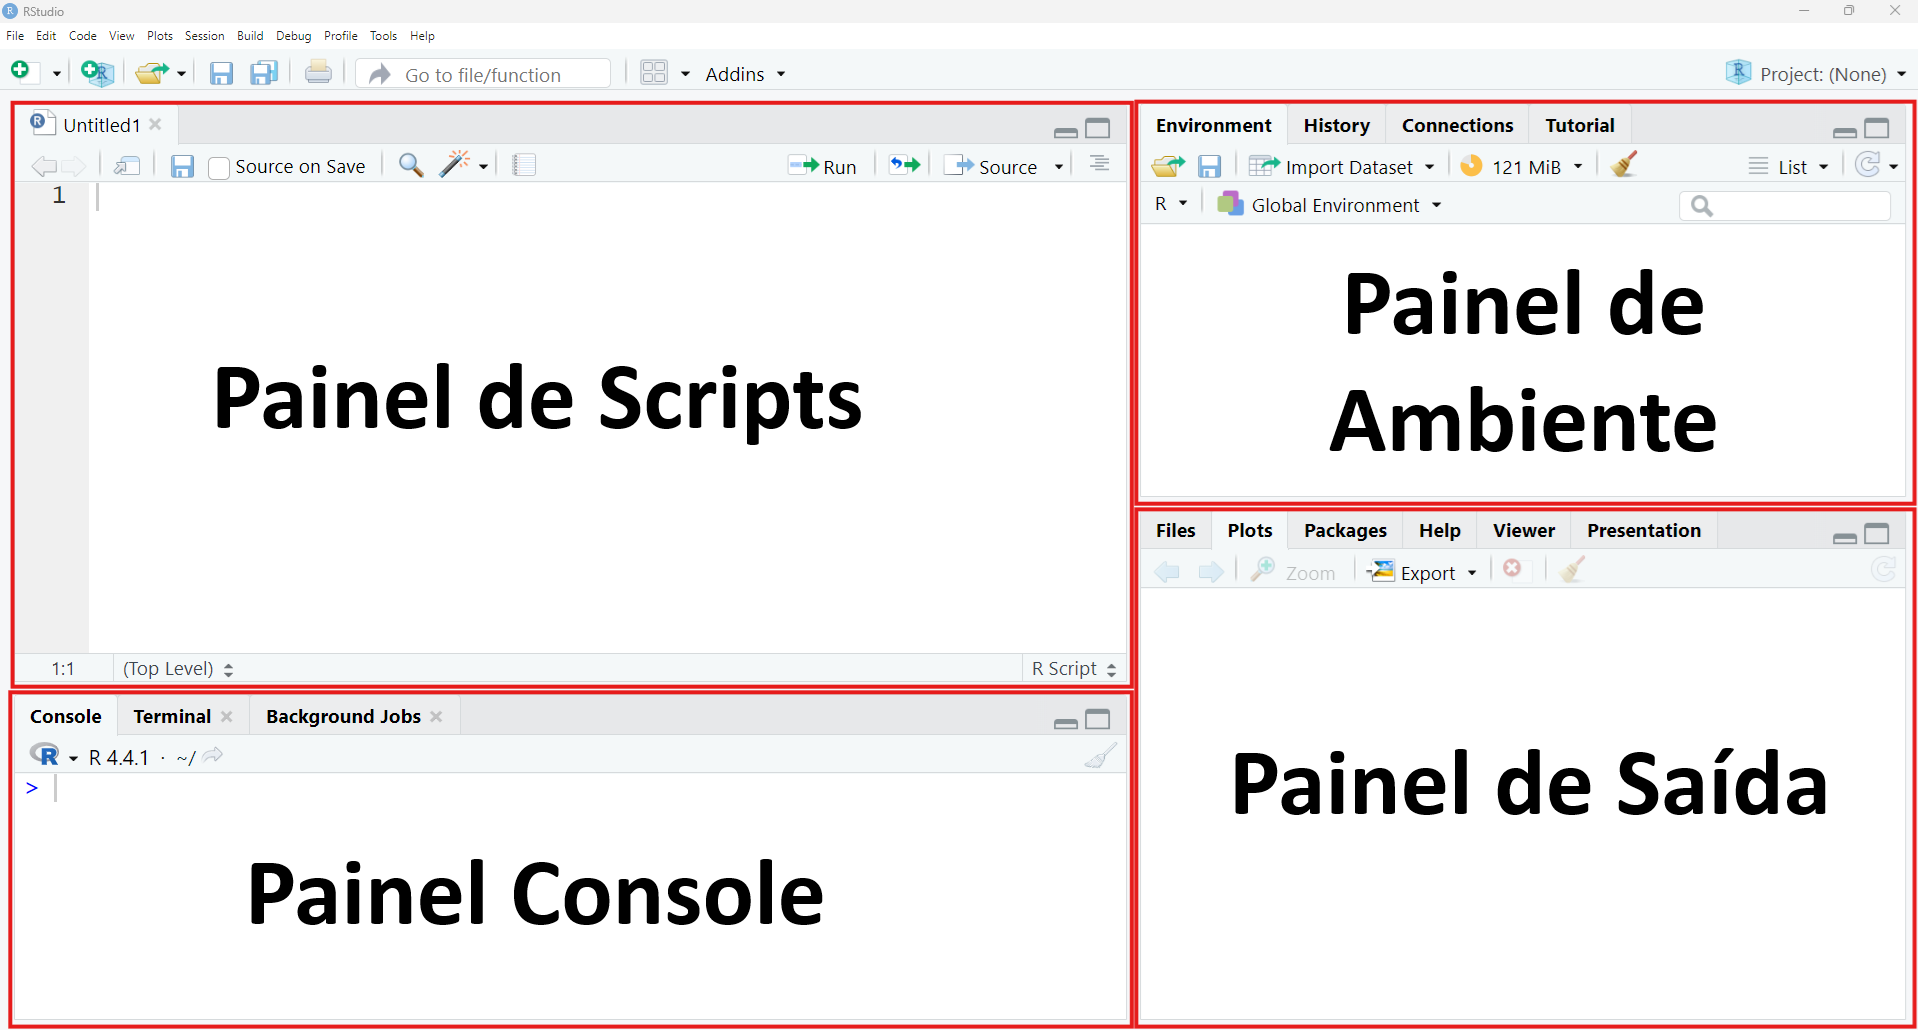
\includegraphics[keepaspectratio]{RStudio_v3.png}}

}

\caption{Figura 01 - Interface do RStudio}

\end{figure}%

\subsection{Painel de Scripts}\label{painel-de-scripts}

Painel onde você pode editar e salvar scripts em R ou criar documentos
computacionais, como Quarto e R Markdown.

\subsection{Painel de Ambiente}\label{painel-de-ambiente}

Painel que exibe os objetos temporários em R à medida que são criados
durante a sessão do R.

\subsection{Painel Console}\label{painel-console}

Painel utilizado para escrever comandos curtos e interativos em R.

\subsection{Painel de Saída}\label{painel-de-sauxedda}

Painel que exibe os gráficos, tabelas ou resultados em HTML gerados pelo
código executado, juntamente com os arquivos salvos em disco.

\section{Regras básicas da sintaxe do
R}\label{regras-buxe1sicas-da-sintaxe-do-r}

A seguir são apresentadas as regras básicas da sintaxe da linguagem R

\subsection{Como atribuir valores a
variáveis}\label{como-atribuir-valores-a-variuxe1veis}

A atribuição de um valor a uma variável é feita através dos operadores
\texttt{\textless{}-} ou \texttt{=}:

\begin{Shaded}
\begin{Highlighting}[]
\NormalTok{x }\OtherTok{\textless{}{-}} \DecValTok{10}
\NormalTok{x }\OtherTok{=} \DecValTok{10}
\end{Highlighting}
\end{Shaded}

\subsection{Sensibilidade a maiúsculas e
minúsculas}\label{sensibilidade-a-maiuxfasculas-e-minuxfasculas}

O R diferencia atributos e nomes de variáveis em letras maiúsculas e
minúsculas:

\begin{Shaded}
\begin{Highlighting}[]
\NormalTok{Altura }\OtherTok{\textless{}{-}} \DecValTok{170}
\NormalTok{altura }\OtherTok{\textless{}{-}} \DecValTok{180}

\FunctionTok{print}\NormalTok{(Altura)}
\end{Highlighting}
\end{Shaded}

\begin{verbatim}
[1] 170
\end{verbatim}

\begin{Shaded}
\begin{Highlighting}[]
\FunctionTok{print}\NormalTok{(altura)}
\end{Highlighting}
\end{Shaded}

\begin{verbatim}
[1] 180
\end{verbatim}

\begin{Shaded}
\begin{Highlighting}[]
\StringTok{"SP"} \SpecialCharTok{==} \StringTok{"sp"}
\end{Highlighting}
\end{Shaded}

\begin{verbatim}
[1] FALSE
\end{verbatim}

\subsection{Como comentar códigos}\label{como-comentar-cuxf3digos}

Os comentários servem como anotações para organizar o código e torná-lo
mais fácil de compreender e replicar. Para inserir um comentário,
utilize o operador \texttt{\#}. Esse operador pode ser utilizado como
cabeçalho para descrever blocos de código, no início de uma linha para
evitar que o código seja executado ou ao final de uma linha de código.
Para comentar um bloco inteiro de código, selecione as linhas desejadas
e pressione \texttt{Crtl} + \texttt{Shift} + \texttt{C}:

\begin{Shaded}
\begin{Highlighting}[]
\CommentTok{\# Vamos agora atribuir o valor 170 para a variável Altura}
\NormalTok{Altura }\OtherTok{\textless{}{-}} \DecValTok{170}

\NormalTok{altura }\OtherTok{\textless{}{-}} \DecValTok{180} \CommentTok{\# Agora atribuímos o valor 180 para a variável altura}

\CommentTok{\# print(altura) \# dessa forma evitamos a impressão do valor da variável.}
\end{Highlighting}
\end{Shaded}

\section{Instalação de pacotes}\label{instalauxe7uxe3o-de-pacotes}

Para instalar pacotes no RStudio, é utilizada a função
\texttt{install.packages()} no console do RStudio:

\begin{Shaded}
\begin{Highlighting}[]
\FunctionTok{install.packages}\NormalTok{()}
\end{Highlighting}
\end{Shaded}

Para instalar diversos pacotes de uma única vez, digite no console do
RStudio a função \texttt{install.packages\ ()} utilizando como argumento
os pacotes \texttt{sf}, \texttt{terra}, \texttt{dplyr},
\texttt{data.table}, \texttt{mapview}, \texttt{osmdata}, \texttt{geobr}
e \texttt{geocodebr}, que são alguns dos pacotes que serão utilizados ao
longo da disciplina:

\begin{Shaded}
\begin{Highlighting}[]
\FunctionTok{install.packages}\NormalTok{(}\FunctionTok{c}\NormalTok{(}\StringTok{"sf"}\NormalTok{, }\StringTok{"terra"}\NormalTok{, }\StringTok{"dplyr"}\NormalTok{, }\StringTok{"data.table"}\NormalTok{, }\StringTok{"mapview"}\NormalTok{, }\StringTok{"osmdata"}\NormalTok{, }\StringTok{"geobr"}\NormalTok{, }\StringTok{"geocodebr"}\NormalTok{))}
\end{Highlighting}
\end{Shaded}

Após instalar os pacotes, carregue-os na sessão atual através da função
\texttt{library()}:

\begin{Shaded}
\begin{Highlighting}[]
\FunctionTok{library}\NormalTok{(sf)}
\end{Highlighting}
\end{Shaded}

\section{Referências:}\label{referuxeancias}

https://docs.posit.co/ide/user/

\bookmarksetup{startatroot}

\chapter{Aula 02}\label{aula-02}

A compatibilização dos sistemas de referencia e das projeções
cartográficas é fundamental para garantir a correta integração de
diferentes dados geoespaciais. Este laboratório didático tem como
objetivo exercitar a identificação de \textbf{Sistemas de Referência de
Coordenadas (CRS)}, a \textbf{transformação entre sistemas de referencia
e a reprojeções de dados geoespaciais}.

\section{\texorpdfstring{\textbf{Sistemas de Referência de Coordenadas
(CRS), transformação entre sistemas de referencia e reprojeções em
R}}{Sistemas de Referência de Coordenadas (CRS), transformação entre sistemas de referencia e reprojeções em R}}\label{sistemas-de-referuxeancia-de-coordenadas-crs-transformauxe7uxe3o-entre-sistemas-de-referencia-e-reprojeuxe7uxf5es-em-r}

\subsection{\texorpdfstring{\textbf{Objetivos de
Aprendizagem}}{Objetivos de Aprendizagem}}\label{objetivos-de-aprendizagem}

\begin{itemize}
\item
  Inspecionar parâmetros dos CRS (Datum, Elipsoide, Unidade e Projeção)
  via código \href{https://epsg.io/}{\textbf{EPSG}}
\item
  Identificar incompatibilidade de CRS entre diferentes fontes de dados
  vetoriais.
\item
  Reprojetar com a função \texttt{st\_transform()}.
\item
  Atribuir CRS com a função \texttt{st\_set\_crs()}.
\end{itemize}

\subsection{\texorpdfstring{\textbf{Roteiro de Execução Passo a
Passo}}{Roteiro de Execução Passo a Passo}}\label{roteiro-de-execuuxe7uxe3o-passo-a-passo}

\subsubsection{\texorpdfstring{\textbf{Preparação do Ambiente no
R}}{Preparação do Ambiente no R}}\label{preparauxe7uxe3o-do-ambiente-no-r}

\begin{Shaded}
\begin{Highlighting}[]
\CommentTok{\# Carregar as bibliotecas fundamentais }
\FunctionTok{library}\NormalTok{(sf)}
\FunctionTok{library}\NormalTok{(dplyr)}
\end{Highlighting}
\end{Shaded}

\subsubsection{\texorpdfstring{\textbf{Leitura do Dado e Inspeção do CRS
Original}}{Leitura do Dado e Inspeção do CRS Original}}\label{leitura-do-dado-e-inspeuxe7uxe3o-do-crs-original}

Baixe os arquivos disponibilizados via Google Classroom e configure o
diretório de trabalho utilizando a função \texttt{setwd()}. Leia o
arquivo \texttt{zonas\_origem\_destino.gpkg} através da função
\texttt{read\_sf()} e inspecione seu CRS por meio da função
\texttt{st\_crs()}:

\begin{Shaded}
\begin{Highlighting}[]
\CommentTok{\# Configuração do diretório de trabalho}
\FunctionTok{setwd}\NormalTok{() }\CommentTok{\# Ajustar para a pasta onde estão localizadas as bases de dados. (p.ex. "C:/Users/User/Downloads/PTR5932\_Lab2")}

\CommentTok{\# Leitura da camada vetorial (GeoPackage) }
\NormalTok{zonas\_sp }\OtherTok{\textless{}{-}} \FunctionTok{read\_sf}\NormalTok{(}\StringTok{"zonas\_origem\_destino.gpkg"}\NormalTok{)  }

\CommentTok{\# Inspeção do CRS da camada }
\FunctionTok{st\_crs}\NormalTok{(zonas\_sp)  }

\CommentTok{\# Extração direta do código EPSG e das unidades de medida planimétricas }
\NormalTok{epsg\_original }\OtherTok{\textless{}{-}} \FunctionTok{st\_crs}\NormalTok{(zonas\_sp)}\SpecialCharTok{$}\NormalTok{epsg }
\NormalTok{unidade\_medida }\OtherTok{\textless{}{-}} \FunctionTok{st\_crs}\NormalTok{(zonas\_sp)}\SpecialCharTok{$}\NormalTok{units\_gdal  }
\FunctionTok{cat}\NormalTok{(}\StringTok{"Código EPSG detectado:"}\NormalTok{, epsg\_original, }\StringTok{"}\SpecialCharTok{\textbackslash{}n}\StringTok{"}\NormalTok{) }
\FunctionTok{cat}\NormalTok{(}\StringTok{"Unidade de medida das coordenadas:"}\NormalTok{, unidade\_medida, }\StringTok{"}\SpecialCharTok{\textbackslash{}n}\StringTok{"}\NormalTok{) }
\end{Highlighting}
\end{Shaded}

\begin{quote}
\textbf{Nota:} A camada está em \textbf{WGS84 Sistema de Coordenadas
Geográficas (EPSG: 4326)}, um dos sistemas de referencia mais utilizados
em dados geoespaciais. O WGS84 é o sistema de referência utilizado pelo
sistema de posicionamento GPS. Nos sistemas de coordenadas geográficas,
as coordenadas são expressas em \emph{graus decimais}.
\end{quote}

\subsubsection{\texorpdfstring{\textbf{Incompatibilidade de
CRS}}{Incompatibilidade de CRS}}\label{incompatibilidade-de-crs}

Carregue a segunda camada (\texttt{estacoes\_metro.gpkg}) e verifique a
compatibilidade entre os CRS:

\begin{Shaded}
\begin{Highlighting}[]
\NormalTok{estacoes }\OtherTok{\textless{}{-}} \FunctionTok{read\_sf}\NormalTok{(}\StringTok{"estacoes\_metro.gpkg"}\NormalTok{)}

\CommentTok{\# Teste lógico de igualdade entre os sistemas de referência }
\ControlFlowTok{if}\NormalTok{ (}\FunctionTok{st\_crs}\NormalTok{(zonas\_sp) }\SpecialCharTok{!=} \FunctionTok{st\_crs}\NormalTok{(estacoes)) \{}\FunctionTok{message}\NormalTok{(}\StringTok{"As camadas possuem CRS distintos e não devem ser sobrepostas sem reprojeção!"}\NormalTok{) \} }
\end{Highlighting}
\end{Shaded}

\begin{quote}
\textbf{Nota:} A camada está em \textbf{Córrego Alegre UTM 23S (EPSG:
22523)}, um sistema de referência geodésico local utilizado
históricamente no Brasil e frequentemente encontrado em dados
cartográficos mais antigos, especialmente extraídos a partir de cartas
topográficas digitalizadas. O Córrego Alegre foi posteriormente
substituído pelo SAD69 e, mais recentemente, pelo SIRGAS2000. Como a
projeção cartográfica adotada é a Universal Transversa de Mercator
(UTM), as coordenadas são expressas em \emph{metros}.
\end{quote}

\subsubsection{\texorpdfstring{\textbf{Transformação Espacial
(Reprojeção)}}{Transformação Espacial (Reprojeção)}}\label{transformauxe7uxe3o-espacial-reprojeuxe7uxe3o}

Para a Região Metropolitana de São Paulo, adotaremos o sistema de
referência projetado \textbf{SIRGAS 2000 / UTM Fuso 23S (EPSG: 31983)},
que utiliza unidades métricas. Para reprojetar os dados, utilize a
função \texttt{st\_transform()}, informando como parâmetros a variável
de entrada e o código EPSG do sistema de referência, \texttt{31983}:

\begin{Shaded}
\begin{Highlighting}[]
\CommentTok{\# Reprojeção da camada de Zonas de Tráfego para SIRGAS 2000 / UTM Fuso 23S }
\NormalTok{zonas\_utm }\OtherTok{\textless{}{-}} \FunctionTok{st\_transform}\NormalTok{(zonas\_sp, }\AttributeTok{crs =} \DecValTok{31983}\NormalTok{)  }

\CommentTok{\# Reprojeção da camada de Estações para SIRGAS 2000 / UTM Fuso 23S }
\NormalTok{estacoes\_utm }\OtherTok{\textless{}{-}} \FunctionTok{st\_transform}\NormalTok{(estacoes, }\AttributeTok{crs =} \DecValTok{31983}\NormalTok{) }

\CommentTok{\# Confirmação do novo CRS }
\FunctionTok{st\_crs}\NormalTok{(zonas\_utm)}\SpecialCharTok{$}\NormalTok{Name }\CommentTok{\# Retorno esperado: "SIRGAS 2000 / UTM zone 23S" }

\CommentTok{\# Confirmação do novo CRS }
\FunctionTok{st\_crs}\NormalTok{(estacoes\_utm)}\SpecialCharTok{$}\NormalTok{Name }\CommentTok{\# Retorno esperado: "SIRGAS 2000 / UTM zone 23S" }
\end{Highlighting}
\end{Shaded}

\subsubsection{\texorpdfstring{\textbf{Atribuição de um sistema de
referência e
projeção}}{Atribuição de um sistema de referência e projeção}}\label{atribuiuxe7uxe3o-de-um-sistema-de-referuxeancia-e-projeuxe7uxe3o}

Caso a camada de entrada não possua um sistema de referência e projeção,
é possível atribuir o CRS adequado à camada, desde que essa informação
seja conhecida previamente, utilizando a função \texttt{st\_set\_crs()}:

\begin{Shaded}
\begin{Highlighting}[]
\CommentTok{\# Leitura da camada de linhas do Metrô de São Paulo}
\NormalTok{linhas\_metro }\OtherTok{\textless{}{-}} \FunctionTok{read\_sf}\NormalTok{(}\StringTok{"linhas\_metro\_SIRGAS2000\_UTM23S.gpkg"}\NormalTok{)}

\CommentTok{\# Consulta do CRS da camada}
\FunctionTok{st\_crs}\NormalTok{(linhas\_metro) }\CommentTok{\#Retorno esperado: NA}

\CommentTok{\# Atribuição do sistema de referência e projeção corretos (baseado no nome da camada)}
\NormalTok{linhas\_metro }\OtherTok{\textless{}{-}}\NormalTok{ linhas\_metro }\SpecialCharTok{\%\textgreater{}\%}
  \FunctionTok{st\_set\_crs}\NormalTok{(}\DecValTok{31983}\NormalTok{)}

\CommentTok{\# Consulta do CRS da camada}
\FunctionTok{st\_crs}\NormalTok{(linhas\_metro)}\SpecialCharTok{$}\NormalTok{Name }\CommentTok{\#Retorno esperado: SIRGAS 2000 / UTM zone 23S}
\end{Highlighting}
\end{Shaded}

\section{Referências:}\label{referuxeancias-1}

https://r-spatial.github.io/sf

https://cran.r-project.org/web/packages/sf/index.html

https://r.geocompx.org/reproj-geo-data

\bookmarksetup{startatroot}

\chapter{Aula 03}\label{aula-03}

Os formatos de representação vetorial e matricial são os mais utilizados
para modelar a realidade. Este laboratório didático possui como objetivo
exercitar a \textbf{leitura, filtragem, relacionamento, criação de novos
campos e a representação de dados vetoriais e matriciais.}

\section{\texorpdfstring{\textbf{Leitura, filtragem, relacionamento,
criação de novos campos e representação de dados vetoriais e
matriciais}}{Leitura, filtragem, relacionamento, criação de novos campos e representação de dados vetoriais e matriciais}}\label{leitura-filtragem-relacionamento-criauxe7uxe3o-de-novos-campos-e-representauxe7uxe3o-de-dados-vetoriais-e-matriciais}

\subsection{\texorpdfstring{\textbf{Objetivos de
Aprendizagem}}{Objetivos de Aprendizagem}}\label{objetivos-de-aprendizagem-1}

\begin{itemize}
\item
  Exercitar a leitura e a filtragem de dados vetoriais através das
  funções \texttt{read\_sf()} e \texttt{filter()}.
\item
  Relacionar a tabela de atributos de um dado vetorial com um tabular
  através da função \texttt{left\_join()}.
\item
  Criar um novo campo com operações matemáticas de campos já existentes
  através da função \texttt{mutate()} e visualizar o dado vetorial
  através da função \texttt{mapview()}.
\item
  Rasterizar um dado vetorial através da função \texttt{rasterize()} e
  visualizá-lo através da função \texttt{plot()}.
\item
  Exportar dados vetoriais e raster, respectivamente, através das
  funções \texttt{write\_sf()} e \texttt{writeRaster()}.
\end{itemize}

\subsection{\texorpdfstring{\textbf{Preparação do Ambiente no
R}}{Preparação do Ambiente no R}}\label{preparauxe7uxe3o-do-ambiente-no-r-1}

\begin{Shaded}
\begin{Highlighting}[]
\CommentTok{\# Carregar as bibliotecas fundamentais }
\FunctionTok{library}\NormalTok{(sf)}
\FunctionTok{library}\NormalTok{(terra)}
\FunctionTok{library}\NormalTok{(dplyr)}
\FunctionTok{library}\NormalTok{(data.table)}
\FunctionTok{library}\NormalTok{(mapview)}
\end{Highlighting}
\end{Shaded}

\subsection{\texorpdfstring{\textbf{Roteiro de Execução Passo a
Passo}}{Roteiro de Execução Passo a Passo}}\label{roteiro-de-execuuxe7uxe3o-passo-a-passo-1}

\subsubsection{\texorpdfstring{\textbf{Leitura e filtragem da base de
dados
vetorial}}{Leitura e filtragem da base de dados vetorial}}\label{leitura-e-filtragem-da-base-de-dados-vetorial}

Baixe os arquivos disponibilizados via Google Classroom e configure o
diretório de trabalho através da função \texttt{setwd()}. Leia o arquivo
\texttt{zonas\_origem\_destino.gpkg} utilizando a função
\texttt{read\_sf()} e filtre somente as zonas OD pertencentes ao
município de São Paulo (código do município == 36) através da função
\texttt{filter()}:

\begin{Shaded}
\begin{Highlighting}[]
\CommentTok{\# Configure o diretório de trabalho}
\FunctionTok{setwd}\NormalTok{() }\CommentTok{\# Ajustar para a pasta onde estão localizadas as bases de dados. (p.ex. "C:/Users/User/Downloads/PTR5932\_Lab3")}

\CommentTok{\# Leia a camada vetorial (GeoPackage) e filtre somente as zonas OD do município de São Paulo }
\NormalTok{zonas\_od }\OtherTok{\textless{}{-}} \FunctionTok{read\_sf}\NormalTok{(}\StringTok{"zonas\_origem\_destino.gpkg"}\NormalTok{) }\SpecialCharTok{\%\textgreater{}\%}
  \FunctionTok{filter}\NormalTok{(cd\_municipio }\SpecialCharTok{==} \DecValTok{36}\NormalTok{)}
\end{Highlighting}
\end{Shaded}

\begin{quote}
\textbf{Nota:} O comando \texttt{\%\textgreater{}\%} e a função
\texttt{filter()} só funcionarão se a biblioteca \texttt{dplyr} tiver
sido carregada.
\end{quote}

\subsubsection{\texorpdfstring{\textbf{Leitura do arquivo tabular e
relacionamento de
tabela}}{Leitura do arquivo tabular e relacionamento de tabela}}\label{leitura-do-arquivo-tabular-e-relacionamento-de-tabela}

Leia o arquivo \texttt{tabela01.csv} através da função \texttt{fread()}.
Em seguida, relacione o dado tabular com o das zonas OD através da
função \texttt{left\_join()}, crie um novo campo com o valor da
densidade de domicilios por hectare através da função \texttt{mutate()}
e visualize os resultados através da função \texttt{mapview()}:

\begin{Shaded}
\begin{Highlighting}[]
\CommentTok{\#Leia o dado tabular}
\NormalTok{tabela01 }\OtherTok{\textless{}{-}} \FunctionTok{fread}\NormalTok{(}\StringTok{"Tabela01.csv"}\NormalTok{, }\AttributeTok{encoding =} \StringTok{"Latin{-}1"}\NormalTok{)}

\CommentTok{\# Relacione a tabela preservando a classe espacial \textquotesingle{}sf\textquotesingle{} }
\NormalTok{zonas\_od\_join }\OtherTok{\textless{}{-}}\NormalTok{ zonas\_od }\SpecialCharTok{\%\textgreater{}\%}
  \FunctionTok{left\_join}\NormalTok{(tabela01, }\AttributeTok{by =} \FunctionTok{c}\NormalTok{(}\StringTok{"cd\_original\_zona\_origem\_destino"}\OtherTok{=}\StringTok{"Zona"}\NormalTok{))}

\CommentTok{\# Crie um campo nomeado "dens\_domicilios" que recebe os valores da divisão dos campos "Domicilios" e "Area\_ha"}
\NormalTok{zonas\_od\_join }\OtherTok{\textless{}{-}}\NormalTok{ zonas\_od\_join }\SpecialCharTok{\%\textgreater{}\%}
  \FunctionTok{mutate}\NormalTok{(}\AttributeTok{dens\_domicilios =}\NormalTok{ Domicilios}\SpecialCharTok{/}\NormalTok{Area\_ha)}

\CommentTok{\# Mude o mapa base da função mapview para imagens de satélite }
\FunctionTok{mapviewOptions}\NormalTok{(}\AttributeTok{basemaps =} \FunctionTok{c}\NormalTok{(}\StringTok{"Esri.WorldImagery"}\NormalTok{, }\StringTok{"OpenTopoMap"}\NormalTok{, }\StringTok{"OpenStreetMap"}\NormalTok{))}

\CommentTok{\# Visualize a variável de domicílios através da função mapview}
\FunctionTok{mapview}\NormalTok{(zonas\_od\_join, }\AttributeTok{zcol =} \StringTok{"dens\_domicilios"}\NormalTok{)}
\end{Highlighting}
\end{Shaded}

\begin{quote}
\textbf{Nota:} Como o dado tabular possui acentos e caracteres
especiais, foi adotado o parâmetro de \texttt{encoding\ =\ Latin-1}
dentro da função \texttt{fread()}.
\end{quote}

\subsubsection{\texorpdfstring{\textbf{Rasterização da camada
vetorial}}{Rasterização da camada vetorial}}\label{rasterizauxe7uxe3o-da-camada-vetorial}

Para rasterizar dados vetoriais, utilize as funções \texttt{rast()} e
\texttt{rasterize()}. Em seguida, visualize o arquivo raster através da
função \texttt{plot()}:

\begin{Shaded}
\begin{Highlighting}[]
\CommentTok{\# crie o arquivo raster de template}
\NormalTok{raster\_template }\OtherTok{\textless{}{-}} \FunctionTok{rast}\NormalTok{(zonas\_od\_join, }\AttributeTok{resolution =} \FloatTok{0.00009}\NormalTok{)}

\CommentTok{\# Execute a rasterização definindo o atributo numérico de interesse }
\NormalTok{raster\_resultado }\OtherTok{\textless{}{-}} \FunctionTok{rasterize}\NormalTok{( }\AttributeTok{x =}\NormalTok{ zonas\_od\_join, }\AttributeTok{y =}\NormalTok{ raster\_template, }\AttributeTok{field =} \StringTok{"dens\_domicilios"}\NormalTok{)}

\CommentTok{\# Visualize o raster gerado}
\FunctionTok{plot}\NormalTok{(raster\_resultado, }\AttributeTok{main =} \StringTok{"Densidade de domicílios por hectare"}\NormalTok{)}
\end{Highlighting}
\end{Shaded}

\subsubsection{\texorpdfstring{\textbf{Exporte arquivos vetoriais e
raster}}{Exporte arquivos vetoriais e raster}}\label{exporte-arquivos-vetoriais-e-raster}

Exporte arquivos vetoriais e raster, respectivamente, através das
funções \texttt{write\_sf()} e \texttt{writeRaster()}:

\begin{Shaded}
\begin{Highlighting}[]
\CommentTok{\# Exporte o dado vetorial utilizando a função write\_sf()}
\FunctionTok{write\_sf}\NormalTok{(zonas\_od\_join, }\StringTok{"zonas\_od\_join.gpkg"}\NormalTok{)}

\CommentTok{\# Exporte o dado raster utilizando a função writeRaster()}
\FunctionTok{writeRaster}\NormalTok{(}\AttributeTok{x =}\NormalTok{ raster\_resultado, }\AttributeTok{filename =} \StringTok{"densidade\_domicilios.tif"}\NormalTok{, }\AttributeTok{filetype =} \StringTok{"GTiff"}\NormalTok{, }\AttributeTok{overwrite =} \ConstantTok{TRUE}\NormalTok{ )}
\end{Highlighting}
\end{Shaded}

\section{Referências:}\label{referuxeancias-2}

https://r-spatial.github.io/sf

\url{https://cran.r-project.org/web/packages/terra/refman/terra.html}

\bookmarksetup{startatroot}

\chapter{Aula 04}\label{aula-04}

A etapa de entrada de dados é fundamental para qualquer projeto em
Ciência de Dados Geoespaciais. A presente aula aborda como importar
algumas das principais fontes de dados espaciais. O conteúdo abrange
análise de topologia e o acesso a bases de dados como a
\textbf{Infraestrutura Nacional de Dados Espaciais (INDE)}, dados de
\textbf{Censos}, \textbf{Geocodificação}, \textbf{OpenStreetMap},
\textbf{Rastreamento} e \textbf{LiDAR}.

\section{\texorpdfstring{\textbf{Acesso e leitura de dados da INDE,
Censos, OpenStreetMap, Geocodificação, Rastreamento e
LiDAR}}{Acesso e leitura de dados da INDE, Censos, OpenStreetMap, Geocodificação, Rastreamento e LiDAR}}\label{acesso-e-leitura-de-dados-da-inde-censos-openstreetmap-geocodificauxe7uxe3o-rastreamento-e-lidar}

\subsection{\texorpdfstring{\textbf{Objetivos de
Aprendizagem}}{Objetivos de Aprendizagem}}\label{objetivos-de-aprendizagem-2}

\begin{itemize}
\item
  Identificar e corrigir erros topológicos.
\item
  Acessar dados da Infraestrutura Nacional de Dados Espaciais (INDE).
\item
  Acessar dados do Censo através dos pacotes \texttt{censobr} e
  \texttt{geobr}.
\item
  Geocodificar uma lista de endereços através do pacote
  \texttt{geocodebr}.
\item
  Acessar dados do OpenStreetMap através do pacote \texttt{osmdata}.
\item
  Ler e tratar dados de rastreamento.
\item
  Ler e tratar dados LiDAR através dos pacotes \texttt{lidR} e
  \texttt{terra}
\end{itemize}

\subsection{\texorpdfstring{\textbf{Preparação do Ambiente no
R}}{Preparação do Ambiente no R}}\label{preparauxe7uxe3o-do-ambiente-no-r-2}

\begin{Shaded}
\begin{Highlighting}[]
\CommentTok{\# Carregar as bibliotecas fundamentais }
\FunctionTok{library}\NormalTok{(sf)          }\CommentTok{\# Manipulação de dados vetoriais (Simple Features)}
\FunctionTok{library}\NormalTok{(tidyverse)   }\CommentTok{\# Manipulação e visualização de dados (dplyr, ggplot2)}
\FunctionTok{library}\NormalTok{(geobr)       }\CommentTok{\# Malhas territoriais oficiais do IBGE}
\FunctionTok{library}\NormalTok{(censobr)     }\CommentTok{\# Microdados e agregados censitários do IBGE}
\FunctionTok{library}\NormalTok{(geocodebr)   }\CommentTok{\# Geocodificação local com base no CNEFE/IBGE}
\FunctionTok{library}\NormalTok{(lwgeom)      }\CommentTok{\# funções para análise topológica}
\FunctionTok{library}\NormalTok{(osmdata)     }\CommentTok{\# Consulta a dados VGI (OpenStreetMap via Overpass API)}
\FunctionTok{library}\NormalTok{(mapview)     }\CommentTok{\# Cartografia temática interativa}
\FunctionTok{library}\NormalTok{(rstudioapi)  }\CommentTok{\# Apontar o diretório de trabalho}
\FunctionTok{library}\NormalTok{(data.table)  }\CommentTok{\# Leitura de dados tabulares}
\FunctionTok{library}\NormalTok{(lidR)        }\CommentTok{\# Leitura de dados LiDAR (LAS/LAZ)}
\FunctionTok{library}\NormalTok{(terra)       }\CommentTok{\# Leitura, tratamento e exportação de dados raster}
\FunctionTok{library}\NormalTok{(rgl)         }\CommentTok{\# Renderização e visualização 3D}

\CommentTok{\#Caso não tenha instalado algum dos pacotes anteriores, execute: }
\CommentTok{\#install.packages("nome do pacote")}

\CommentTok{\# Configure o diretório de trabalho}
\NormalTok{path }\OtherTok{\textless{}{-}} \FunctionTok{selectDirectory}\NormalTok{(}\AttributeTok{caption =} \StringTok{"Select Working Directory"}\NormalTok{) }\CommentTok{\# rode esta linha para apontar o diretório de trabalho}

\FunctionTok{setwd}\NormalTok{(path)}
\FunctionTok{mapviewOptions}\NormalTok{(}\AttributeTok{basemaps =} \FunctionTok{c}\NormalTok{(}\StringTok{"Esri.WorldImagery"}\NormalTok{, }\StringTok{"OpenTopoMap"}\NormalTok{, }\StringTok{"OpenStreetMap"}\NormalTok{))}
\end{Highlighting}
\end{Shaded}

\begin{quote}
\textbf{Nota:} O comando \texttt{selectDirectory()} abre uma interface
para que o usuário indique o diretório de trabalho.
\end{quote}

\subsection{\texorpdfstring{\textbf{Roteiro de Execução Passo a
Passo}}{Roteiro de Execução Passo a Passo}}\label{roteiro-de-execuuxe7uxe3o-passo-a-passo-2}

\subsubsection{\texorpdfstring{\textbf{Análise topológica das Zonas OD
2023 de São
Paulo}}{Análise topológica das Zonas OD 2023 de São Paulo}}\label{anuxe1lise-topoluxf3gica-das-zonas-od-2023-de-suxe3o-paulo}

Quando trabalhamos com dados geoespaciais vetoriais, é essencial
verificarmos a sua consistência topológica. Inconsistências topológicas,
como auto-intersecções (\emph{self-intersections}), sobreposições
indevidas (\emph{overlaps}) e lacunas não planejadas (\emph{gaps}) entre
polígonos adjacentes, podem comprometer a precisão de análises
territoriais, distorcer cálculos de área e provocar falhas na execução
de operações espaciais. O script abaixo utiliza os pacotes \texttt{sf} e
\texttt{lwgeom}, para identificar e corrigir automaticamente falhas
topológicas em camadas vetoriais de polígonos:

\begin{Shaded}
\begin{Highlighting}[]
\CommentTok{\# Ler arquivo shapefile das Zonas OD 2023 disponibilizado pelo Metrô }
\NormalTok{zonas\_od }\OtherTok{\textless{}{-}} \FunctionTok{read\_sf}\NormalTok{(}\StringTok{"Zonas\_2023.shp"}\NormalTok{, }\AttributeTok{options =} \StringTok{"ENCODING=LATIN1"}\NormalTok{) }

\CommentTok{\# Verificar se existem geometrias inválidas }
\NormalTok{zonas\_od}\SpecialCharTok{$}\NormalTok{valido }\OtherTok{\textless{}{-}} \FunctionTok{st\_is\_valid}\NormalTok{(zonas\_od) }

\CommentTok{\# Contar de geometrias válidas e inválidas }
\FunctionTok{table}\NormalTok{(zonas\_od}\SpecialCharTok{$}\NormalTok{valido) }

\CommentTok{\# Identificar o motivo exato de cada invalidade }
\NormalTok{zonas\_od}\SpecialCharTok{$}\NormalTok{motivo\_erro }\OtherTok{\textless{}{-}} \FunctionTok{st\_is\_valid}\NormalTok{(zonas\_od, }\AttributeTok{reason =} \ConstantTok{TRUE}\NormalTok{) }

\CommentTok{\# Listar os tipos de erros encontrados no dataset e armazená{-}los em uma variável. Inspecionar os erros após rodar a linha abaixo}
\NormalTok{erros }\OtherTok{\textless{}{-}}\NormalTok{ zonas\_od }\SpecialCharTok{\%\textgreater{}\%} 
  \FunctionTok{filter}\NormalTok{(}\SpecialCharTok{!}\NormalTok{valido) }\SpecialCharTok{\%\textgreater{}\%} 
  \FunctionTok{st\_drop\_geometry}\NormalTok{() }\SpecialCharTok{\%\textgreater{}\%} 
  \FunctionTok{count}\NormalTok{(motivo\_erro, }\AttributeTok{sort =} \ConstantTok{TRUE}\NormalTok{)}

\CommentTok{\# Aplicar a correção automáticamente}
\NormalTok{zonas\_od\_corrigidas }\OtherTok{\textless{}{-}} \FunctionTok{st\_make\_valid}\NormalTok{(zonas\_od)}

\CommentTok{\# Verificar se ainda são encotradas geometrias inválidas }
\NormalTok{zonas\_od\_corrigidas}\SpecialCharTok{$}\NormalTok{valido }\OtherTok{\textless{}{-}} \FunctionTok{st\_is\_valid}\NormalTok{(zonas\_od\_corrigidas) }

\CommentTok{\# Contar geometrias válidas e inválidas }
\FunctionTok{table}\NormalTok{(zonas\_od\_corrigidas}\SpecialCharTok{$}\NormalTok{valido) }

\CommentTok{\# Visualizar as Zonas OD de 2023}
\FunctionTok{mapview}\NormalTok{(zonas\_od\_corrigidas) }
\end{Highlighting}
\end{Shaded}

\begin{quote}
\textbf{Nota:} Os erros mais comuns, do tipo ``Self-intersection'',
ocorrem quando a linha de contorno da zona cruza consigo mesma formando
um laço.
\end{quote}

\subsubsection{\texorpdfstring{\textbf{Acesso a Infraestrutura Nacional
de Dados Espaciais
(INDE)}}{Acesso a Infraestrutura Nacional de Dados Espaciais (INDE)}}\label{acesso-a-infraestrutura-nacional-de-dados-espaciais-inde}

A INDE concentra o acesso a diversas bases de dados oficiais de orgãos
do governo. No exemplo abaixo, acessaremos o serviço de WFS (Web Feature
Service), por onde são disponibilizados dados vetoriais. Para isso,
indique a URL do serviço WFS, liste as camadas existentes e faça a
leitura da camada de arruamento utilizando a função \texttt{st\_read()}.
Em seguida, inspecione o sistema de referência e a projeção cartográfica
da base de dados de arruamento e, caso seja necessário, faça os devidos
ajustes. Por fim, visualize a base de dados através da função
\texttt{mapview()}, diferenciando o arruamento de acordo com seu
revestimento:

\begin{Shaded}
\begin{Highlighting}[]
\CommentTok{\# Consumo de uma camada WFS (Web Feature Service) da INDE}
\NormalTok{url\_wfs }\OtherTok{\textless{}{-}} \FunctionTok{sprintf}\NormalTok{(}\StringTok{"https://geoservicos.inde.gov.br/geoserver/wfs"}\NormalTok{) }\CommentTok{\# Exemplo conceitual de endpoint WFS}

\CommentTok{\#info\_camadas \textless{}{-} st\_layers(paste0("WFS:", url\_wfs)) \# Lista as camadas do WFS, porém para a INDE fica muito demorado, pois são muitas camadas. }

\CommentTok{\# Leitura direta de camada espacial vetorial via protocolo OGC WFS sem download manual}
\CommentTok{\# sf permite conexão direta com URLs WFS/GeoJSON da INDE}
\NormalTok{IDE\_camada }\OtherTok{\textless{}{-}} \FunctionTok{st\_read}\NormalTok{(}\AttributeTok{dsn =} \FunctionTok{paste0}\NormalTok{(url\_wfs, }\StringTok{"?service=WFS\&version=1.0.0\&request=GetFeature\&typeName=INEA:gln\_arruamento\_25\_armacao\_dos\_buzios"}\NormalTok{))}

\CommentTok{\# Inspeção do Sistema de Referência de Coordenadas (CRS / SIRGAS 2000 {-} EPSG:4674)}
\FunctionTok{st\_crs}\NormalTok{(IDE\_camada)}

\NormalTok{IDE\_camada }\OtherTok{\textless{}{-}} \FunctionTok{st\_set\_crs}\NormalTok{(IDE\_camada, }\DecValTok{4674}\NormalTok{)}
\FunctionTok{st\_crs}\NormalTok{(IDE\_camada)}

\FunctionTok{mapviewOptions}\NormalTok{(}\AttributeTok{basemaps =} \FunctionTok{c}\NormalTok{(}\StringTok{"Esri.WorldImagery"}\NormalTok{, }\StringTok{"OpenTopoMap"}\NormalTok{, }\StringTok{"OpenStreetMap"}\NormalTok{))}

\NormalTok{mapview}\SpecialCharTok{::}\FunctionTok{mapview}\NormalTok{(IDE\_camada, }\AttributeTok{zcol =} \StringTok{"revestimen"}\NormalTok{)}
\end{Highlighting}
\end{Shaded}

\begin{quote}
\textbf{Nota:} Foi atribuído o EPSG 4674, pois todos os dados
disponibilizados através da INDE estão no referencial SIRGAS2000 e em
Sistemas de Coordenadas Geográficas.
\end{quote}

\subsubsection{\texorpdfstring{\textbf{Acesso a dados do Censo
Demográfico}}{Acesso a dados do Censo Demográfico}}\label{acesso-a-dados-do-censo-demogruxe1fico}

Serão utilizados os pacotes \texttt{geobr} e \texttt{censobr} para
baixar, respectivamente, os dados espaciais e os dados tabulares dos
setores censitários. Em seguida, os dados são relacionados através da
função \texttt{left\_join()} e visualizados através da função
\texttt{mapview()}:

\begin{Shaded}
\begin{Highlighting}[]
\CommentTok{\# Download da malha de setores censitários de um município (ex: Armação de Búzios/RJ) via geobr}
\NormalTok{setores\_ab }\OtherTok{\textless{}{-}} \FunctionTok{read\_census\_tract}\NormalTok{(}\AttributeTok{year =} \DecValTok{2022}\NormalTok{, }\AttributeTok{code\_tract =} \DecValTok{3300233}\NormalTok{)}
\FunctionTok{st\_crs}\NormalTok{(setores\_ab)}

\CommentTok{\# Leitura dos dados do Censo 2022 agregados por Setor Censitário via censobr}
\NormalTok{dados\_setores }\OtherTok{\textless{}{-}} \FunctionTok{read\_tracts}\NormalTok{(}\AttributeTok{year =} \DecValTok{2022}\NormalTok{, }\AttributeTok{dataset =} \StringTok{"Basico"}\NormalTok{) }\SpecialCharTok{\%\textgreater{}\%}
  \FunctionTok{filter}\NormalTok{(code\_muni }\SpecialCharTok{==} \DecValTok{3300233}\NormalTok{) }\SpecialCharTok{\%\textgreater{}\%} \CommentTok{\# filtra apenas o município de Armação de Búzios/RJ}
  \FunctionTok{collect}\NormalTok{() }\CommentTok{\# Traz para a memória o resultado filtrado}

\FunctionTok{data\_dictionary}\NormalTok{(}\AttributeTok{year =} \DecValTok{2022}\NormalTok{, }\AttributeTok{dataset =} \StringTok{"tracts"}\NormalTok{) }\CommentTok{\# dicionario de dados para verificar os nomes das variaveis e sua descrição}

\NormalTok{dados\_setores }\OtherTok{\textless{}{-}}\NormalTok{ dados\_setores }\SpecialCharTok{\%\textgreater{}\%}
  \FunctionTok{select}\NormalTok{(code\_tract, V0001) }\CommentTok{\# seleciona apenas as variaveis de código do setor (code\_tract) e População total (V001)}

\NormalTok{setores\_ab\_join }\OtherTok{\textless{}{-}}\NormalTok{ setores\_ab }\SpecialCharTok{\%\textgreater{}\%}
  \FunctionTok{left\_join}\NormalTok{(dados\_setores, }\AttributeTok{by=}\StringTok{"code\_tract"}\NormalTok{) }\CommentTok{\#join do dado espacial de setores censitários com o dado de população}

\CommentTok{\# Visualizacao dos dados de população por setor censitário de 2022}
\FunctionTok{mapview}\NormalTok{(setores\_ab\_join, }\AttributeTok{zcol =} \StringTok{"V0001"}\NormalTok{)}
\end{Highlighting}
\end{Shaded}

\begin{quote}
\textbf{Nota:} Na função \texttt{read\_tracts()} foi selecionado o
dataset ``Basico''. No entanto, existem ainda os datasets ``Pessoas'',
``Domicilios'', ``Obitos'', ``Indigenas'', ``Quilombolas'',
``ResponsavelRenda'' e ``Entorno'', ou seja, existem muitos outros dados
a serem explorados.
\end{quote}

\subsubsection{\texorpdfstring{\textbf{Geocodificação}}{Geocodificação}}\label{geocodificauxe7uxe3o}

A geocodificação consiste em transformar um endereço (ou lista de
endereços) em um par (ou vários pares) de coordenadas. A geocodificação
pode ser realizada gratuitamente através do pacote \texttt{geocodebr}:

\begin{Shaded}
\begin{Highlighting}[]
\CommentTok{\# Leitura da lista de endereços para geocodificação}
\NormalTok{enderecos }\OtherTok{\textless{}{-}} \FunctionTok{fread}\NormalTok{(}\StringTok{"RMSPEstb\_2014\_10000reg.csv"}\NormalTok{)}
  
\CommentTok{\# Mapeamento dos campos com definir\_campos()}
\NormalTok{campos }\OtherTok{\textless{}{-}} \FunctionTok{definir\_campos}\NormalTok{(}
  \AttributeTok{logradouro =} \StringTok{"nomelogradouro"}\NormalTok{,}
  \AttributeTok{numero =} \StringTok{"numero"}\NormalTok{,}
  \AttributeTok{municipio =} \StringTok{"municipio"}\NormalTok{,}
  \AttributeTok{estado =} \StringTok{"uf"}\NormalTok{)}

\CommentTok{\# 3. Execução da geocodificação via geocodebr}
\NormalTok{resultados\_geocod }\OtherTok{\textless{}{-}} \FunctionTok{geocode}\NormalTok{(}
  \AttributeTok{enderecos =}\NormalTok{ enderecos,}
  \AttributeTok{campos\_endereco =}\NormalTok{ campos}
\NormalTok{)}

\CommentTok{\# O resultado retorna com níveis de precisão da geocodificação, longitude e latitude }
\FunctionTok{head}\NormalTok{(resultados\_geocod)}

\CommentTok{\# Espacialização dos resultados}
\NormalTok{resultados\_geocod\_sf }\OtherTok{\textless{}{-}} \FunctionTok{st\_as\_sf}\NormalTok{(resultados\_geocod, }\AttributeTok{coords =} \FunctionTok{c}\NormalTok{(}\StringTok{"lon"}\NormalTok{, }\StringTok{"lat"}\NormalTok{), }\AttributeTok{crs =} \DecValTok{4674}\NormalTok{)}

\CommentTok{\# Visualização dos resultados de acordo com a precisão da geocodificação}
\FunctionTok{mapview}\NormalTok{(resultados\_geocod\_sf, }\AttributeTok{zcol =} \StringTok{"precisao"}\NormalTok{)}
\end{Highlighting}
\end{Shaded}

\subsubsection{\texorpdfstring{\textbf{Acesso aos dados do
OSM}}{Acesso aos dados do OSM}}\label{acesso-aos-dados-do-osm}

Uma fonte importante de dados espaciais são os mapeamentos
colaborativos. Na área de transportes, uma das principais iniciativas é
o OpenStreetMap (OSM), que disponibiliza informações sobre a rede viária
em escala mundial. Os dados do OSM podem ser acessados através do pacote
\texttt{osmdata}:

\begin{Shaded}
\begin{Highlighting}[]
\CommentTok{\# Definição da caixa delimitadora (Bounding Box)}
\NormalTok{bb }\OtherTok{\textless{}{-}} \FunctionTok{opq}\NormalTok{(}\AttributeTok{bbox =} \StringTok{"São Paulo, Brasil"}\NormalTok{)}

\CommentTok{\# Consulta à API Overpass para extrair ciclovias (cycleways)}
\NormalTok{ciclovias }\OtherTok{\textless{}{-}}\NormalTok{ bb }\SpecialCharTok{\%\textgreater{}\%}
  \FunctionTok{add\_osm\_feature}\NormalTok{(}\AttributeTok{key =} \StringTok{"highway"}\NormalTok{, }\AttributeTok{value =} \StringTok{"cycleway"}\NormalTok{) }\SpecialCharTok{\%\textgreater{}\%}
  \FunctionTok{osmdata\_sf}\NormalTok{()}

\CommentTok{\# Extração das geometrias do tipo linha}
\NormalTok{linhas\_ciclovias }\OtherTok{\textless{}{-}}\NormalTok{ ciclovias}\SpecialCharTok{$}\NormalTok{osm\_lines}

\CommentTok{\# Visualização das ciclovias classificadas pelo atributo de segregação (parâmetro zcol)}
\FunctionTok{mapviewOptions}\NormalTok{(}\AttributeTok{basemaps =} \FunctionTok{c}\NormalTok{(}\StringTok{"Esri.WorldImagery"}\NormalTok{, }\StringTok{"OpenTopoMap"}\NormalTok{, }\StringTok{"OpenStreetMap"}\NormalTok{))}
\FunctionTok{mapview}\NormalTok{(linhas\_ciclovias, }\AttributeTok{zcol =} \StringTok{"segregated"}\NormalTok{) }
\end{Highlighting}
\end{Shaded}

\subsubsection{\texorpdfstring{\textbf{Dados de
rastreamento}}{Dados de rastreamento}}\label{dados-de-rastreamento}

Outra fonte abundante de dados espaciais, principalmente na área de
transportes, são os dados de rastreamento. Esses dados são normalmente
obtidos a partir do rastreamento de receptores GNSS, que podem estar
acoplados a veículos ou a qualquer outro objeto de interesse. Os dados
de rastreamento podem apresentar formatos heterogêneos, mas precisam
conter, no mínimo, latitude, longitude, data (dia, mês e ano) e horário
do registro. A seguir, apresenta-se um exemplo de espacialização de uma
base de dados de rastreamento de ônibus:

\begin{Shaded}
\begin{Highlighting}[]
\CommentTok{\# Leitura da base de dados de rastreamento de ônibus da SPTrans (Linha 34831)}
\NormalTok{ rastreio }\OtherTok{\textless{}{-}} \FunctionTok{fread}\NormalTok{(}\StringTok{"rastreio\_linha34831\_data\_01\_03\_2015.csv"}\NormalTok{)}

\CommentTok{\# Dicionario de dados:}
 \CommentTok{\#V1 = \textquotesingle{}dataserver\textquotesingle{}}
 \CommentTok{\#V2 = \textquotesingle{}dataavl\textquotesingle{}}
 \CommentTok{\#V3 = \textquotesingle{}linha\textquotesingle{} }
 \CommentTok{\#V4 = \textquotesingle{}lat\textquotesingle{}}
 \CommentTok{\#V5 = \textquotesingle{}lon\textquotesingle{} }
 \CommentTok{\#V6 = \textquotesingle{}codavl\textquotesingle{} }
 \CommentTok{\#V7 = \textquotesingle{}desc1\textquotesingle{} }
 \CommentTok{\#V8 = \textquotesingle{}desc2\textquotesingle{}}
 
\CommentTok{\# Espacialização da base de dados de rastreamento}
\NormalTok{rastreio\_espacializado }\OtherTok{\textless{}{-}}\NormalTok{ rastreio }\SpecialCharTok{\%\textgreater{}\%}
  \FunctionTok{st\_as\_sf}\NormalTok{(}\AttributeTok{coords =} \FunctionTok{c}\NormalTok{(}\StringTok{"V5"}\NormalTok{, }\StringTok{"V4"}\NormalTok{), }\AttributeTok{crs =} \DecValTok{4326}\NormalTok{) }

\CommentTok{\# Visualização da base de dados}
\FunctionTok{mapview}\NormalTok{(rastreio\_filtro)}
\end{Highlighting}
\end{Shaded}

\subsubsection{\texorpdfstring{\textbf{Dados
LiDAR}}{Dados LiDAR}}\label{dados-lidar}

Por fim, dados espaciais provenientes de levantamentos com sensores
LiDAR tem sido encontrados cada vez mais frequentemente em estudos
urbanos. Os sensores LiDAR podem ser acoplados a diferentes tipos de
plataformas e constituem uma fonte rica de dados para extrair
informações sobre a cobertura da superfície e gerar Modelos Digitais de
Elevação. Os dados LiDAR podem ser lidos e processados através dos
pacotes \texttt{lidR}, \texttt{rgl} e \texttt{terra}:

\begin{Shaded}
\begin{Highlighting}[]
\CommentTok{\# Ler o arquivo LAZ }
\NormalTok{las }\OtherTok{\textless{}{-}} \FunctionTok{readLAS}\NormalTok{(}\StringTok{"MDS\_3313{-}152\_1000.laz"}\NormalTok{) }

\CommentTok{\# Validar e inspecionar os metadados da nuvem (densidade de pontos, atributos) }
\FunctionTok{print}\NormalTok{(las) }

\CommentTok{\# Checar a integridade da geometria da nuvem }
\FunctionTok{las\_check}\NormalTok{(las) }

\CommentTok{\# Visualização 3D da Nuvem de Pontos Original }
\FunctionTok{plot}\NormalTok{(las, }\AttributeTok{color =} \StringTok{"Z"}\NormalTok{, }\AttributeTok{bg =} \StringTok{"black"}\NormalTok{, }\AttributeTok{axis =} \ConstantTok{TRUE}\NormalTok{) }

\CommentTok{\# Filtragem dos pontos classificados como Terreno (Padrão ASPRS: Classe 2 = Terreno).}
\NormalTok{las\_terreno }\OtherTok{\textless{}{-}} \FunctionTok{filter\_ground}\NormalTok{(las) }

\CommentTok{\# Visualizar apenas a nuvem filtrada do solo em 3D }
\FunctionTok{plot}\NormalTok{(las\_terreno, }\AttributeTok{color =} \StringTok{"Z"}\NormalTok{, }\AttributeTok{bg =} \StringTok{"white"}\NormalTok{) }

\CommentTok{\# Geração do Modelo Digital do Terreno (MDT / DTM) }
\NormalTok{mdt }\OtherTok{\textless{}{-}} \FunctionTok{rasterize\_terrain}\NormalTok{( }
  \AttributeTok{las =}\NormalTok{ las\_terreno, }
  \AttributeTok{res =} \FloatTok{0.5}\NormalTok{, }\CommentTok{\# Resolução espacial da célula (ex: 1 metro) }
  \AttributeTok{algorithm =} \FunctionTok{tin}\NormalTok{() }\CommentTok{\# Algoritmo de interpolação por Triangulação Delaunay }
\NormalTok{  ) }

\CommentTok{\# Plotagem 2D do MDT gerado (objeto SpatRaster do pacote \textquotesingle{}terra\textquotesingle{}) }
\FunctionTok{plot}\NormalTok{(mdt, }\AttributeTok{main =} \StringTok{"Modelo Digital do Terreno (MDT) {-} Resolução: 1m"}\NormalTok{, }\AttributeTok{col =} \FunctionTok{terrain.colors}\NormalTok{(}\DecValTok{50}\NormalTok{)) }

\CommentTok{\# Exportar o raster resultante para formato GeoTIFF }
\FunctionTok{writeRaster}\NormalTok{(mdt, }\AttributeTok{filename =} \StringTok{"MDT.tif"}\NormalTok{, }\AttributeTok{overwrite =} \ConstantTok{TRUE}\NormalTok{)}
\end{Highlighting}
\end{Shaded}

\section{Referências:}\label{referuxeancias-3}

https://r-spatial.github.io/sf

\url{https://cran.r-project.org/web/packages/censobr/vignettes/censobr.html}

\url{https://cran.r-project.org/web/packages/geobr/index.html}

\url{https://cran.r-project.org/web/packages/geocodebr/index.html}

\url{https://cran.r-project.org/web/packages/osmdata/index.html}

\url{https://cran.r-project.org/web/packages/lidR/index.html}

\url{https://cran.r-project.org/web/packages/rgl/index.html}

\url{https://cran.r-project.org/web/packages/terra/refman/terra.html}

\bookmarksetup{startatroot}

\chapter*{Referências}\label{referuxeancias-4}
\addcontentsline{toc}{chapter}{Referências}

\markboth{Referências}{Referências}

BURROUGH, P. A.; MCDONNELL, R. A. Principles of geographical information
systems. New York: Oxford University Press, 1998. 334p.

DE SMITH, M. J.; GOODCHILD, M. F.; LONGLEY, P. Geospatial analysis: a
comprehensive guide to principles, techniques and software tools.
Troubador Publishing Ltd, 2025 - 7th edition. Disponível em:
http://www.spatialanalysisonline.com/HTML/index.html

GEMAEL, C. Introdução à Geodésia Física. Editora da UFPR. Curitiba,
1999.

HOFMANN-WELLENHOF, B.; LICHTENEGGER, H.; WASLE, E. GNSS: Global
Navigation Satellite Systems -- GPS, GLONASS, Galileo \& more. Austria:
Springer-Verlag Wien New York, 1a edição, 2008. 516p. ISBN
978-3-211-73012-6

LOVELACE, R.; NOWOSAD, J.; MUENCHOW, J.Geocomputation with R. Chapman
and Hall/CRC, 2025. Disponível em: https://doi.org/10.1201/9780203730058

MACLACHLAN, A.; DENNETT, A. An Applied Geographic Information Systems
and Science Course in R.Journal of Open Source Education, v. 5, n.~50,
2022. Disponível em: https://doi.org/10.21105/jose.00141

MONICO, J. F. G. Posicionamento pelo GNSS: Descrição, fundamentos e
aplicações. São Paulo, Editora UNESP, 2007. 476p. ISBN:
978-85-7139-788-0

PEREIRA, R. H.; SARAIVA, M.; HERSZENHUT, D.; BRAGA, C. K. V.; CONWAY, M.
W. r5r: rapid realistic routing on multimodal transport networks with r
5 in r.\emph{Findings}, 2021. https://doi.org/10.32866/001c.21262

RICHARDUS, P.; ADLER, R.K. Map Projections for Geodesists, Cartographers
and Geographers. North-Holland Publishing Company, 1972.

TEAM, R. Core. R language definition.Vienna, Austria: R foundation for
statistical computing, v. 3, n.~1, p.~116, 2000.
https://mirror.twds.com.tw/CRAN/doc/FAQ/r-release/R-lang.pdf




\end{document}
